\chapter{Implementation}
This chapter is split into three main sections:


\begin{itemize}
\item Technologies Used
\end{itemize}

Both the software and hardware used in the development for both RideSafe \& the companion data collection variant.



\begin{itemize}
\item Main Activities
\end{itemize}



The main activity implementations will be discussed in detail along with their underlying purpose. 

\begin{itemize}
\item Training
\end{itemize}


The methods used to train RideSafe’s Multivariate logistic regression model will be explained in terms of how and where the data was recorded.


\section{Technologies Used}
This section will discuss the technologies used in the development of RideSafe.

\subsection{Android}

%%%%%%%%%%%%%%%%%%%%%%%%%%%%%%%%%%%%%%%%
\begin{wrapfigure}{r}{0.1\textwidth}
\begin{center}

\includegraphics[scale = 0.3] {implementation/android.jpg}
\end{center}

\label{android}
\end{wrapfigure}
%%%%%%%%%%%%%%%%%%%%%%%%%%%%%%%%%%%%%%%%

Android was chosen as the target platform for numerous reasons:
\begin{itemize}
\item previous Experience 
\end{itemize}
The author currently owning multiple android devices as well as having previous experience developing small scale android apps, Android was the clear target for development.  Usually deemed as less intuitive to develop the author was unfazed due to previous experience.

\vspace{2cm}

\begin{itemize}
\item Market Share/Target Audience 
\end{itemize}
%%%%%%%%%%%%%%%%%%%%%%%%%%%%%%%%%%%%%%%%
\begin{figure}
\begin{center}
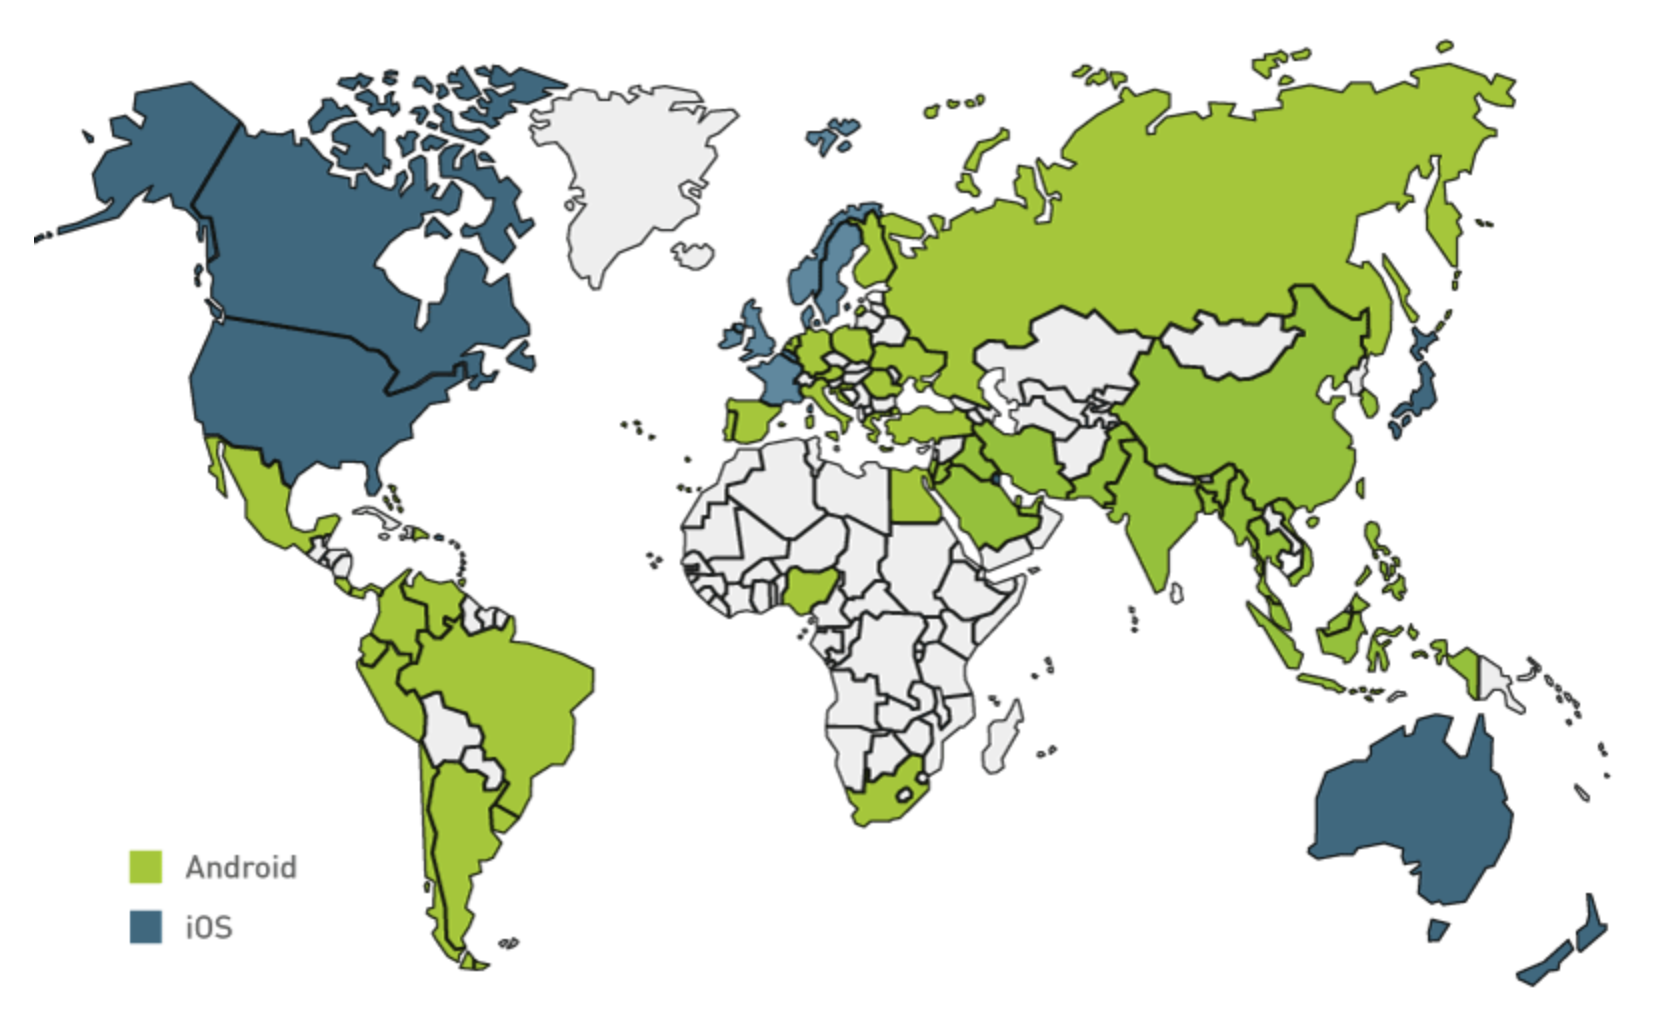
\includegraphics[scale = 0.4] {implementation/marketshare.png}
\end{center}
\caption{Market share (source: App Annie)}
\label{MAP}
\end{figure}
%%%%%%%%%%%%%%%%%%%%%%%%%%%%%%%%%%%%%%%%

Currently there are more active android devices than there are ios devices globally. Knowing real world tests would be required from willing participants, the likelihood of them owning an android device would be marginally higher.
\begin{itemize}
\item Access to hardware
\end{itemize}

The most important factor, Android allows for much better access to the hardware of the device it is installed on, crucial for an application relying on accurate and reliable sensor measurements. Being a less restrictive unix based operating system features such as file management are also possible. The offloading of sensor readings is a simple process through any pc or another android device.


\subsection{Android Studio - Java}

%%%%%%%%%%%%%%%%%%%%%%%%%%%%%%%%%%%%%%%%
\begin{wrapfigure}{l}{0.4\textwidth}
\begin{center}

\includegraphics[scale = 0.3] {implementation/studio-logo.png}
\end{center}

\label{studio}
\end{wrapfigure}
%%%%%%%%%%%%%%%%%%%%%%%%%%%%%%%%%%%%%%%%

Android Studio, being the official IDE for developing android applications and being provided by Google, it was the clear choice. As well as including Github integration for easy version control, Android studio includes useful debugging features such as logcat to view exactly what line of code in which file caused an error. The built in AVD manager allows for testing of code in an emulated android environment, this proved useful for ui changes but does not include sensors or gps leading me to do most of my testing on my own device. Android Studio’s profiler proved useful to help me stay on track in terms of power consumption. Resources such as memory and cpu usage can be monitored on a per activity basis, which ultimately led to some code restructuring to improve device responsiveness in some situations. Android runs java natively, allowing some aspects such as the Logistic Regression class to be developed, tested and optimized on a desktop computer, which with little effort can be copied into the application where it will perform as expected. Investigating the ideal learning rate and number of iterations were also conducted on a computer, which saved a lot of time compiling the application and installing it every time a change was made.   



\subsection{SQLite}

%%%%%%%%%%%%%%%%%%%%%%%%%%%%%%%%%%%%%%%%
\begin{wrapfigure}{r}{0.4\textwidth}
\begin{center}

\includegraphics[scale = 0.5] {implementation/SQLite.png}
\end{center}

\label{sql}
\end{wrapfigure}
%%%%%%%%%%%%%%%%%%%%%%%%%%%%%%%%%%%%%%%%





Databases are crucial to the functionally of RideSafe, using SQLite databases in android allow for secure reliable data Storage. Separate tables contain data such as training data and profile information, crucial datasets for the apps operation.  The usage of cursors allow for easy navigation and data retrieval. The use of a databaseHelper class allowed for the use of simple java functions to perform complex SQL commands, which removed the need to write raw SQL commands more than once.

\subsection{Github}
%%%%%%%%%%%%%%%%%%%%%%%%%%%%%%%%%%%%%%%%
\begin{wrapfigure}{l}{0.5\textwidth}
\begin{center}

\includegraphics[scale = 0.4] {implementation/github.png}
\end{center}

\label{git}
\end{wrapfigure}
%%%%%%%%%%%%%%%%%%%%%%%%%%%%%%%%%%%%%%%%




Github was used for version control for both RideSafe and the data collection app. Github served as a secure backup of work and allowed the author to switch between desktops and laptops in seconds, continuing from exactly where they left off. Branching allowed for major changes with the option to revert back to a working state easily if necessary. Both RideSafe and the data collection version both share a large portion of code, copying the repo and uploading it under a different name when development required allowed for both apps to be developed essentially in parallel and when the time came both apps could be developed separately.   


\subsection{Python}
%%%%%%%%%%%%%%%%%%%%%%%%%%%%%%%%%%%%%%%%
\begin{wrapfigure}{r}{0.5\textwidth}
\begin{center}

\includegraphics[scale = 0.5] {implementation/python-logo.png}
\end{center}

\label{python}
\end{wrapfigure}
%%%%%%%%%%%%%%%%%%%%%%%%%%%%%%%%%%%%%%%%

The source code for RideSafe does not contain a single line of python, however the functions provided in google sheets were limiting what operations that could be done to sort the raw sensor data that was collected. Using python thousands of lines of raw sensor data could be processed and categorized in an instant, ultimately allowing the charastics of crashes to be learnt by analysing sorted data. File combinations also were handled in python, depending on use RideSafe Data Collection App would export multiple files of different runs or one single file with hours of non related data also included. The use of python allowed for hours of manual sorting to be done automatically in seconds.


\section{Main Activities}

This section will discuss in detail the main activities and classes used in the main operation of RideSafe
\subsection{Splash Screen \& Logistic Regression}

%%%%%%%%%%%%%%%%%%%%%%%%%%%%%%%%%%%%%%%%
\begin{wrapfigure}{r}{0.3\textwidth}
\begin{center}
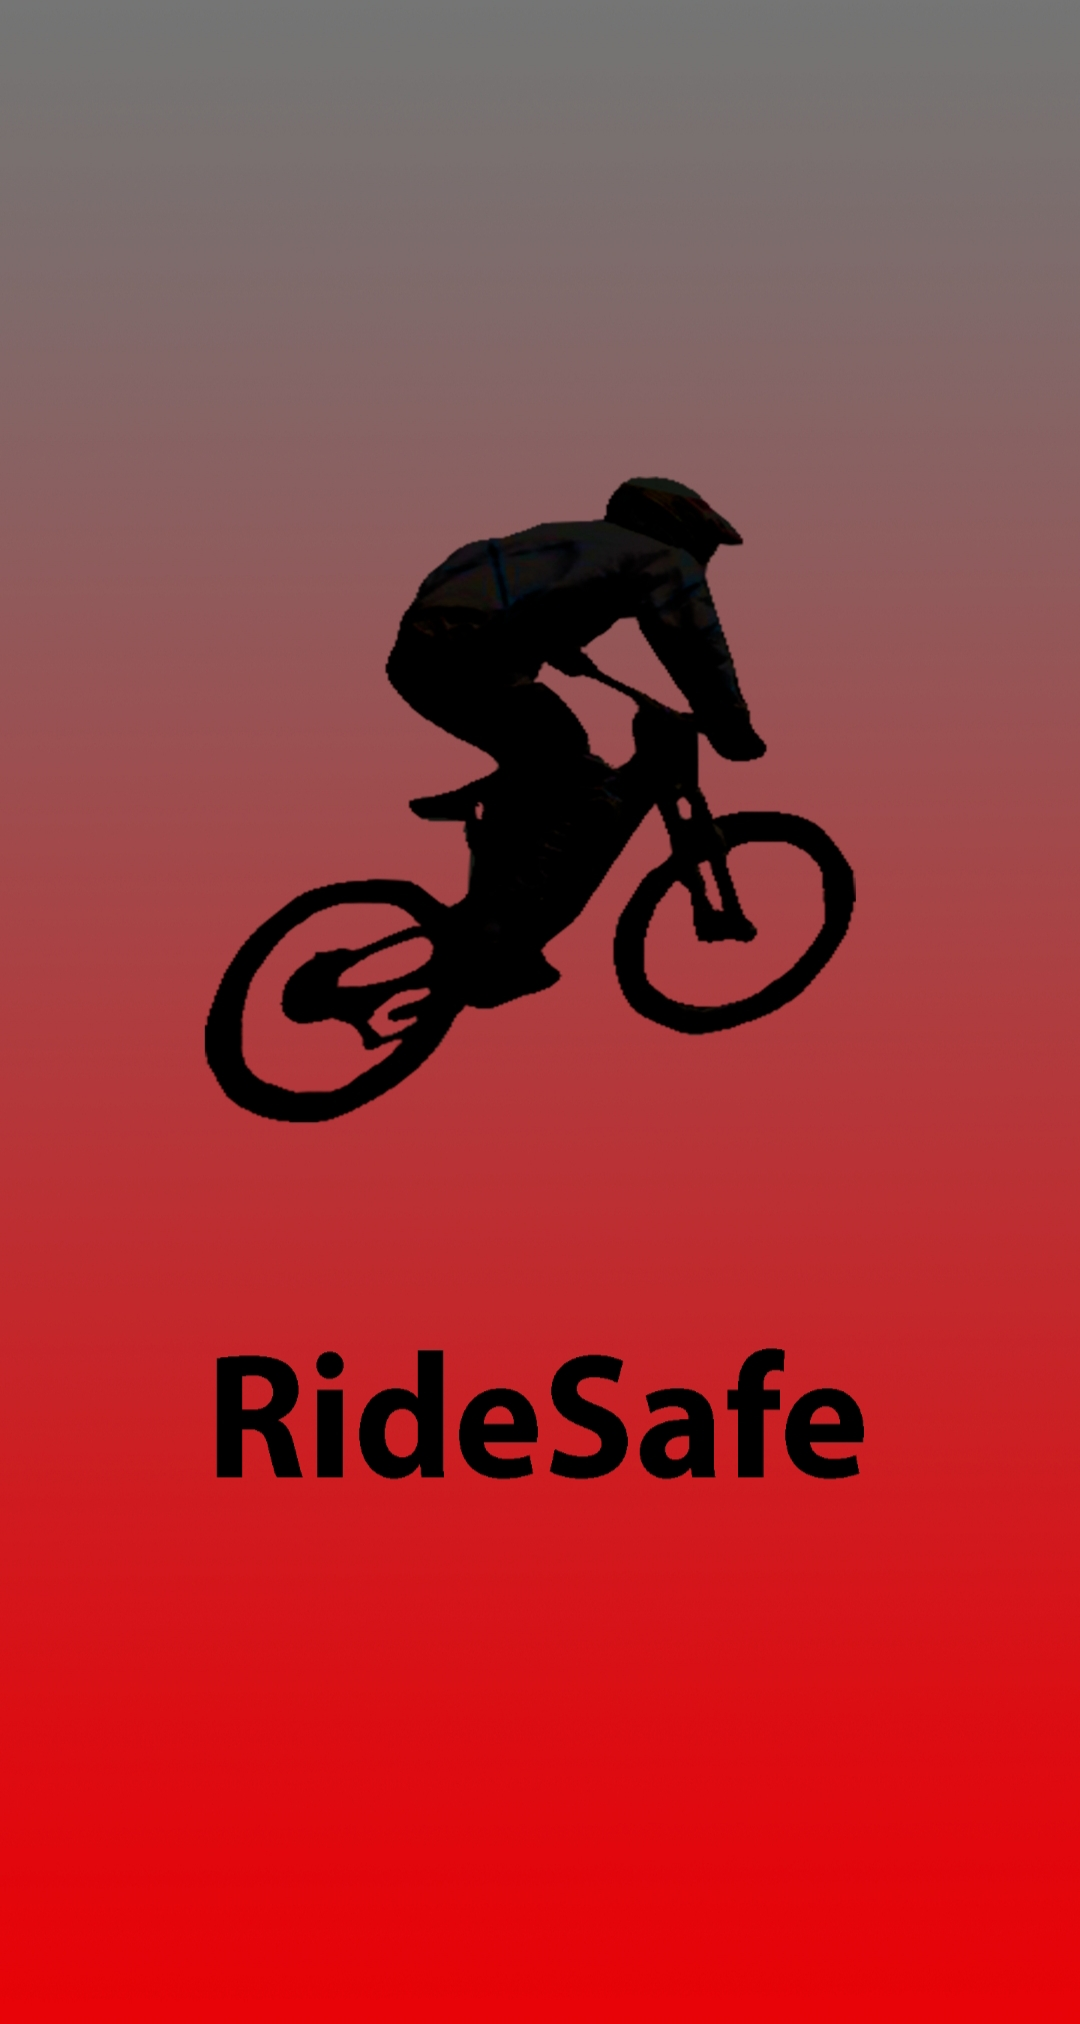
\includegraphics[scale = 0.1] {implementation/splash.jpg}
\end{center}
\caption{A Screenshot of the Slash Screen}
\label{splash}
\end{wrapfigure}
%%%%%%%%%%%%%%%%%%%%%%%%%%%%%%%%%%%%%%%%


To the user the splash screen looks to be simply a loading image as seen in Figure \ref{splash} , but this is not the case. In the background some operations crucial to operation are being carried out. Firstly RideSafe checks if the application has previously been set up by means of a SQLite query, by querying the number of entries of the user profile table, the requirement for setup being required can be determined. If setup is required RideSafe directs the user through the setup process.

\vspace{3cm}


\begin{lstlisting}[language=Java,basicstyle=\small, breaklines=true, label={lst:Code Snippet1},caption={Querying database entries}]
SQLiteDatabase db = mDatabaseHelper.getWritableDatabase();
int tableRows = (int) DatabaseUtils
.queryNumEntries(db, "profile_info");
if (tableRows < 1)
\end{lstlisting}






For performance and stability reasons two major tasks are also run: 



\begin{itemize}
\item{Loading and updating training data.}
\end{itemize}

In the case of either the app is run for the first time or an updated version of the training data is pushed, the training data will be reloaded. The training data supplied with ridesafe is stored as an asset as a text file, the text file, shown in figure \ref{std}, contains the known sensor values of both crashes and normal riding. The final column is the label for the data, used to indicate whether the data corresponds to a crash (1) or a non crash (0). Loading data from a file is expensive in terms of time, so this process is only performed when absolutely necessary. The training data is read in line by line and stored in a SQLite database table. The data provides secure storage and quick access to the data when needed.


%%%%%%%%%%%%%%%%%%%%%%%%%%%%%%%%%%%%%%%%
\begin{figure}[h]
      \centering
      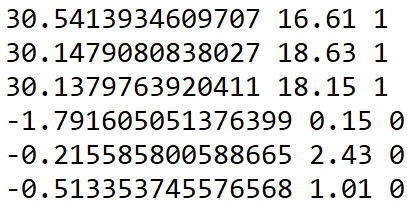
\includegraphics[scale = 1]{implementation/std.png}
      \caption{An Example Of RideSafe Training Data}
      \label{std}
\end{figure}
%%%%%%%%%%%%%%%%%%%%%%%%%%%%%%%%%%%%%%%%

\vspace{1cm}

\begin{lstlisting}[language=Java,basicstyle=\small, breaklines=true, label={lst:labell},caption={Loading Training Data from a file and storing in a database table}]
try (BufferedReader reader = new BufferedReader(
	new InputStreamReader(getAssets().open("TrainingData.txt")))) {
	
	// loop untill eof
	String mLine;
	while ((mLine = reader.readLine()) != null) {
		String[] columns = mLine.split("\\s+");
		double[] data = new double[columns.length];
		for (int i = 0; i < columns.length; i++) {
		data[i] = Double.parseDouble(columns[i]);
                }
           
		ContentValues values = new ContentValues();
		values.put("gforce", data[0]);
		values.put("rotation", data[1]);
		values.put("label",data[2]);
		mDatabaseHelper.addRow(values, "TrainingData");
\end{lstlisting}




\begin{itemize}
\item  {Training the logistic regression model.}
\end{itemize}


Once the data has been loaded for the first time or updated the logistic model needs to be re trained. Testing had shown a very small learning rate of 0.0005 combined with 500 iterations calculated accurate weights for each variable in a training data set containing circa 300 entries. Training data used for Ridesafe will be discussed in section 4.3. A combination of a small learning rate paired with a large number of weight estimate iterations ensures accurate weights can be calculated. In this implementation the weights are along a u-shaped curve, using the learning rate as essentially a step size increases the accuracy of weight estimation. The learning rate can be observed as linearly dependant in respect to the iteration count. If a very large learning rate was used the algorithm could overstep or undershoot  the most accurate weight estimation. The implications of using too few iterations would result in the system terminating prematurely, resulting in incomplete weight estimations.




\begin{lstlisting}[language=Java,basicstyle=\small, breaklines=true, label={lst:train},caption={Training/updating the Model}]
  public void train(DatabaseHelper mDatabaseHelper, int col) {
        Cursor dataCursor = mDatabaseHelper.getData("td");
        int numRows = 0;
        while (dataCursor.moveToNext()){
            numRows++;
        }
        for (int n=0; n<numIterations; n++) {
            dataCursor.moveToFirst();
            for (int i=0; i<numRows; i++) {
                double[] x;
                x = new double[1];
                x[0] = dataCursor.getDouble(col);
                double predicted = classify(x);
                double DataLabel = dataCursor.getInt(3);
                weights[0] = weights[0] + LearningRate * (DataLabel - predicted) * x[0];
                dataCursor.moveToNext();
            }
        }
        System.out.println( Arrays.toString(weights) );
        dataCursor.close();
    }
\end{lstlisting}




Figure \ref{std} shows an example of RideSafes training data, the first column is g-force, followed by change in rotational velocity and finally the assigned label.
For each row in the training data training table of the database,  the value is classified based on the current calculated weight (var predicted). Then the weight for that sensor reading is recalculated based on what the system has already learnt, with the exception of iteration 0 where the predicted value will be 50\% likely. 
  weights[i] = weights[i] + Learning Rate * (DataLabel - predicted) * x[i];
The current weight for sensor data i = the current weight for sensor data i + the specified learning rate(0.0005) * (The known class of the variable either 1 for a crash or 0 otherwise - what it currently classifies as) * the sensor reading associated with that weight. This process is repeated until the weights are as accurate as possible and no longer change. The final calculated Weights for both g-force \& total rotational velocity change from the training data used can be seen in figure \ref{weights}. The regression model provides an answer to the following in real-time, Given current sensor values x , what is the probability of (1|x) where 1 is the class label belonging to data pre-learnt of accidents.




%%%%%%%%%%%%%%%%%%%%%%%%%%%%%%%%%%%%%%%%
\begin{figure}[h]
      \centering
      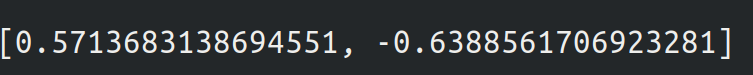
\includegraphics[scale = .5]{implementation/weights.png}
      \caption{Weights calculated by the Multivariate Logistic Model}
      \label{weights}
\end{figure}
%%%%%%%%%%%%%%%%%%%%%%%%%%%%%%%%%%%%%%%%

\vspace{2cm}

The function used for classification as shown below is an implementation of the formula for the sigmoidal Logistic curve  \[
    P = \frac{1}{1+e^ -(a+bX)}
\]   For Each Row of data the probability P is calculated using the logistic curve.


\begin{lstlisting}[language=Java,basicstyle=\small, breaklines=true, label={lst:labell},caption={Classify Function}]

 public double classify(double[] x) {
        double logit = .0;
        for (int i=0; i<weights.length;i++)  {
            logit += weights[i] * x[i];
        }
        return 1.0 / (1.0 + Math.exp(-logit));
    }
\end{lstlisting}





As seen in figure \ref{logit} green points on the graph are plotted with a probability near 0, these points represent the sensor values associated with a non crash. The red points are plotted probabilities of sensor values representing crashes. The blue point represents classified sensor values with no known truth, using the learnt weights the model calculates the probability of the likelihood the readings match those of an accident, e, g,. The sensor values related to the blue dot are more similar to what the system knows is a crash, resulting in a high probability that a crash has occurred. 






%%%%%%%%%%%%%%%%%%%%%%%%%%%%%%%%%%%%%%%%
\begin{figure}[h]
      \centering
      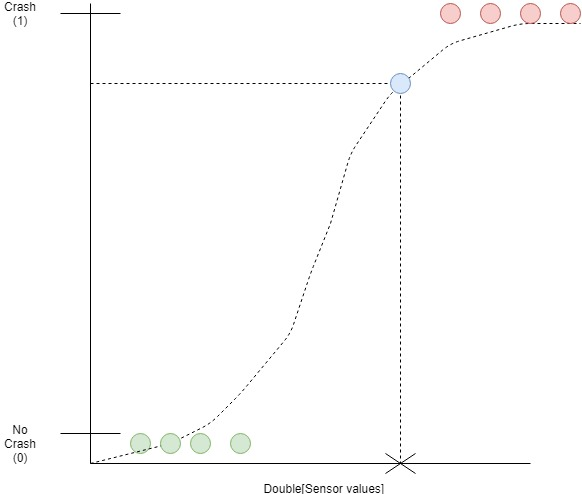
\includegraphics[scale = .6]{implementation/logit.jpg}
      \caption{Sigmoid curve produced by a logit function}
      \label{logit}
\end{figure}
%%%%%%%%%%%%%%%%%%%%%%%%%%%%%%%%%%%%%%%%


\vspace{3cm}




%%%%%%%%%%%%%%%%%%%%%%%%%%%%%%%%%%%%%%%%
\begin{figure}[h]
      \centering
      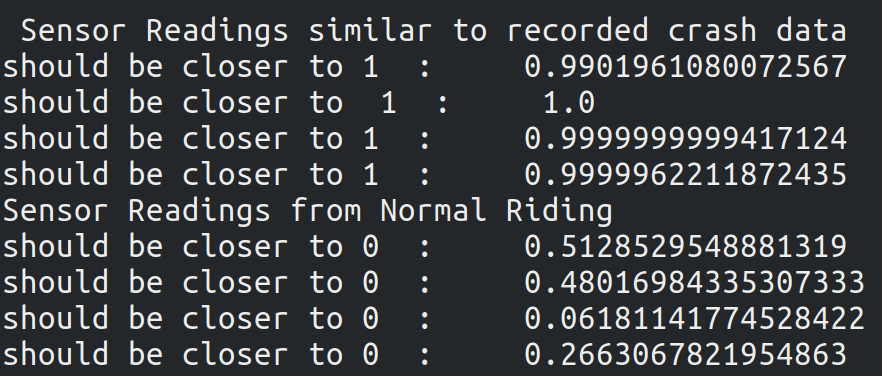
\includegraphics[scale = .5]{implementation/tv.png}
      \caption{Classifying Example Test values With A Trained Model}
      \label{tv}
\end{figure}
%%%%%%%%%%%%%%%%%%%%%%%%%%%%%%%%%%%%%%%%



Figure \ref{tv} shows example test cases of both crash and non crash data being classified, Crash data is quite unique versus standard riding data leading to crashes being identified to a high degree of certainty, Normal Riding varies quite a lot leading to a range of output probabilities. 



\newpage
\subsection{Home Screen}


%%%%%%%%%%%%%%%%%%%%%%%%%%%%%%%%%%%%%%%%
\begin{wrapfigure}{r}{0.3\textwidth}
\begin{center}
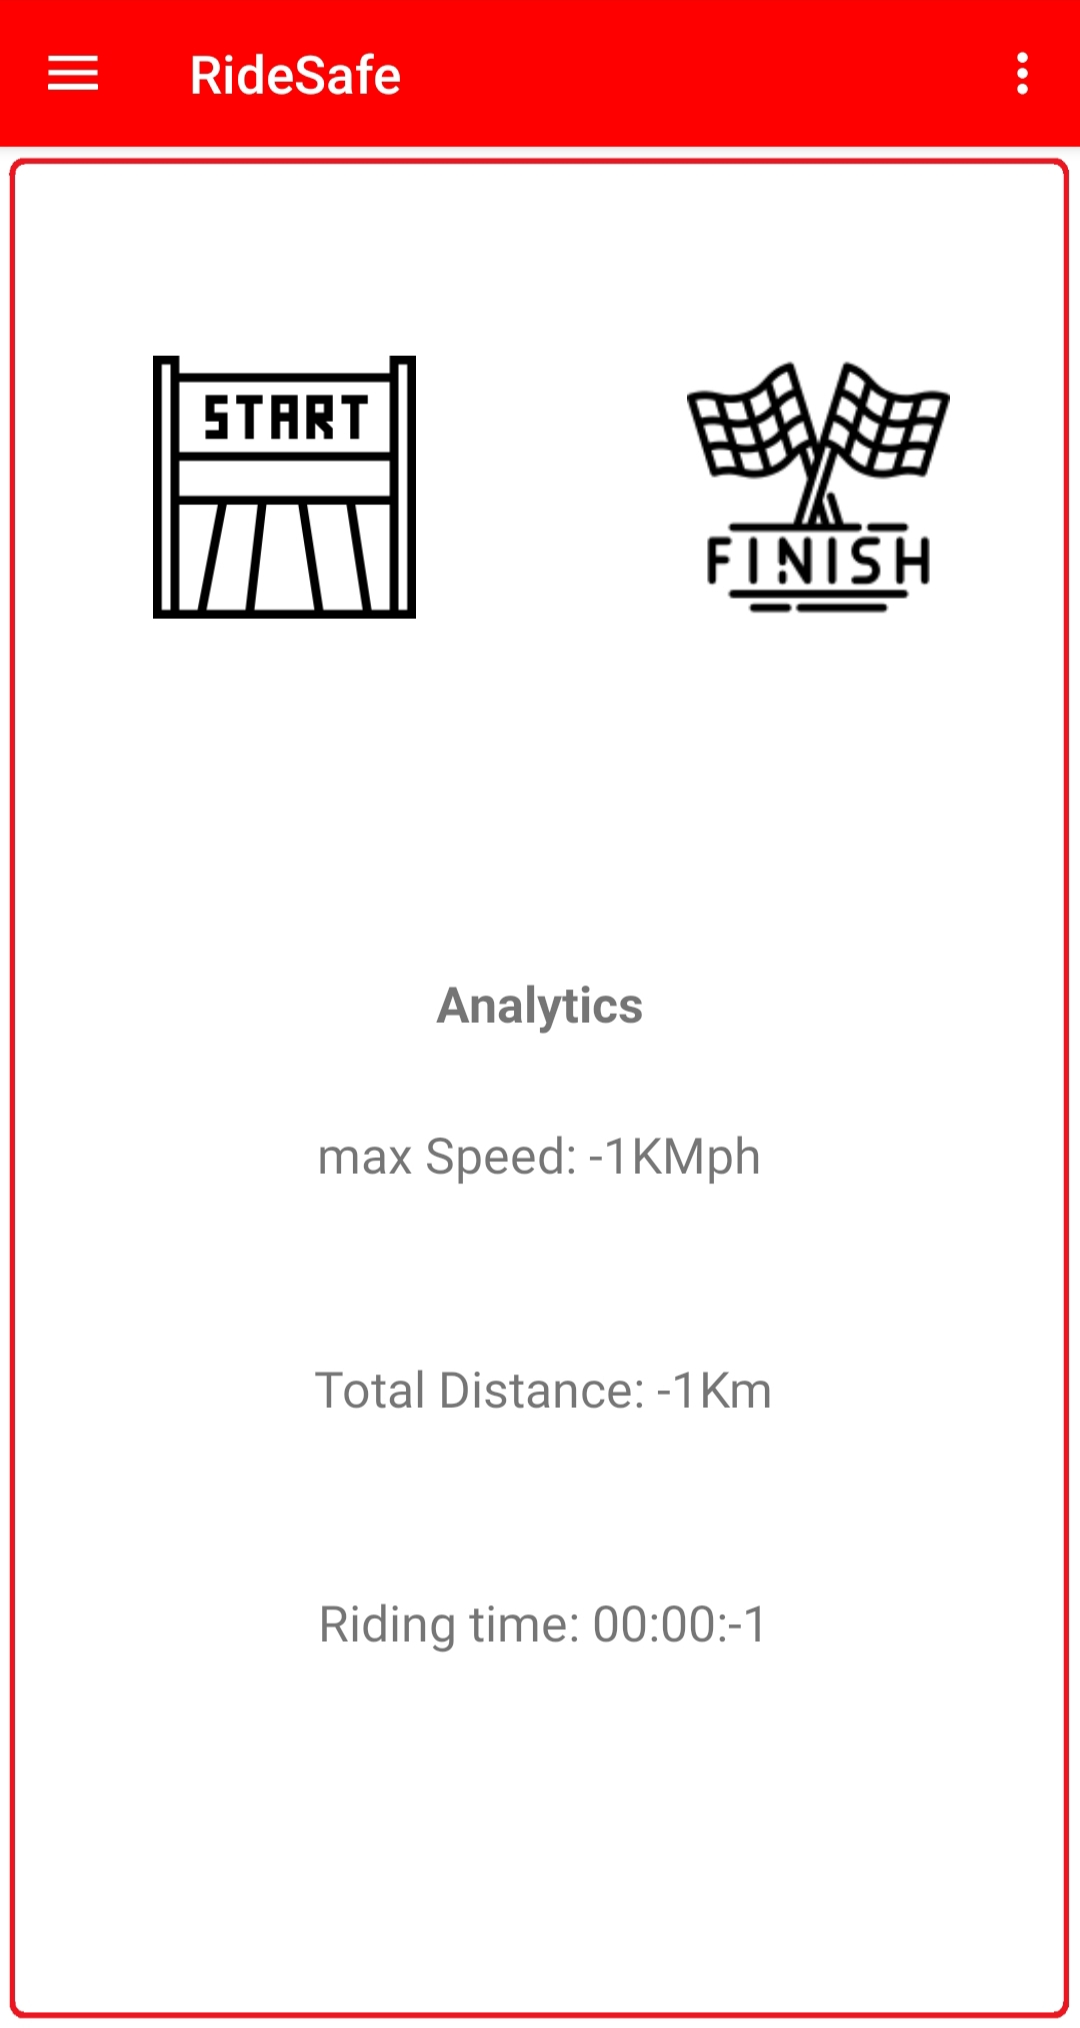
\includegraphics[scale = 0.15] {implementation/home.jpg}
\end{center}
\caption{A Screenshot of the home Screen}
\label{homescreen}
\end{wrapfigure}
%%%%%%%%%%%%%%%%%%%%%%%%%%%%%%%%%%%%%%%%


The author kept the home screen as simple and user friendly as possible. By utilizing large black icons against a plain white background the screen remains viewable in extremely bright and dark environments. Buttons were kept large for ease of use while wearing gloves as many cyclists do. Towards the bottom of the screen are some useful analytics for the user such as their max recorded speed \& distance traveled. 


\begin{lstlisting}[language=Java,basicstyle=\small, breaklines=true, label={lst:labellll},caption={Starting the Crash Detection Service}]

public void startService(View v) {

        locationManager = (LocationManager) getSystemService(LOCATION_SERVICE);
        gpsManager = new GPSConfig(main_Home.this);
        isGPSon = locationManager.isProviderEnabled(LocationManager.GPS_PROVIDER);

        if (isGPSon) {
            String init = "running";
            Intent serviceIntent = new Intent(this, RideSafeService.class);
            serviceIntent.putExtra("inputExtra", init);
            startService(serviceIntent);
            RUNNING = true;
        } else {
            showSettingsAlert();
        }
    }
\end{lstlisting}

On Pressing the Start Button RideSafe performs a check to determine if location services are enabled for the device. If GPS is not enabled the user is prompted to do so in their device settings, otherwise an intent is launched to start the background service which will be discussed in detail in the next section. 
The Stop service button is simply the opposite of the start button bar the gps check, An intent is launched on pressing the to end the background service. The analytics section is also updated on pressing finish.  










\subsection{RideSafe Background Service}

%%%%%%%%%%%%%%%%%%%%%%%%%%%%%%%%%%%%%%%%
\begin{wrapfigure}{r}{0.2\textwidth}
\begin{center}
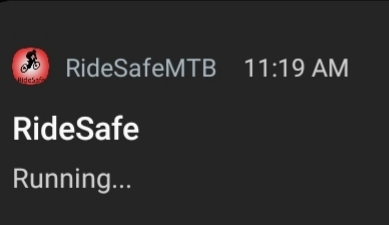
\includegraphics[scale = 0.2] {implementation/service.jpg}
\end{center}
\caption{A Screenshot of the service notification}
\label{crash}
\end{wrapfigure}
%%%%%%%%%%%%%%%%%%%%%%%%%%%%%%%%%%%%%%%%

RideSafes background service is where both all the sensor monitoring takes place and the rule based system is implemented. On pressing the start button on the home screen the background service is launched. This background service has no view or user interface layout, the user is reassured the system is running  with a persistent device notification which can be seen in figure (ref), Google recently required any background service to have a notification displayed to inform the user operations are being performed which cannot be seen.



 \begin{lstlisting}[language=Java,basicstyle=\small, breaklines=true, label={lst:labell},caption={Taking Sensor Readings}]

@Override
    public void onSensorChanged(SensorEvent event) {

        sensorType = event.sensor.getType();
        if (sensorType == 1 && !GAquired) {     // accelerometer
            X = event.values[0];
            Y = event.values[1];
            Z = event.values[2];
            ACCELEROMETER = Math.sqrt(X * X + Y * Y + Z * Z) - 9.807;
            ACCELEROMETER = (double)Math.round(ACCELEROMETER * 100d)/100d;
            GAquired = true;

            if(RAquired) {
                GAquired = false;
                RAquired = false;
                ClassifyX();
            }
        } else if (sensorType != 1 && !RAquired) {

            GYROX = event.values[0];
            GYROY = event.values[1];
            GYROZ = event.values[2];

            GYROX = (double)Math.round(event.values[0] * 100d)/100d;
            GYROY = (double)Math.round(event.values[1] * 100d)/100d;
            GYROZ = (double)Math.round(event.values[2] * 100d)/100d;
            currentRot = GYROX + GYROY + GYROZ / 3;
            currentRot = (double)Math.round(currentRot * 100d)/100d;

            RAquired = true;
            if(GAquired){
                GAquired = false;
                RAquired = false;
                ClassifyX();
            }

        }
    }

\end{lstlisting}



 \begin{lstlisting}[language=Java,basicstyle=\small, breaklines=true, label={lst:labell},caption={Senor Setup}]


SM.registerListener(this, myAccelerometer, SensorManager.SENSOR_DELAY_NORMAL);
        SM.registerListener(this, myGyroscope, SensorManager.SENSOR_DELAY_NORMAL);

\end{lstlisting}



The recording of sensor values is performed as shown above in lstlisting Sensor Readings In the onCreate method both the accelerometer and gyroscope are initialized as well as registering device listeners. As both sensors are required to use the same onsensorchanged method booleans are used as triggers similar to the operation of a basic state machine. When readings from both sensors have been acquired they are converted into the required format as discussed previously in the design section. The next reading required is the current speed.


 \begin{lstlisting}[language=Java,basicstyle=\small, breaklines=true, label={lst:labell},caption={Calculating Speed \& Distance}]


@Override
    public void onGPSUpdate(Location location) {
        speed = location.getSpeed();
        currentSpeed = round(speed, 3, BigDecimal.ROUND_HALF_UP);
        SPEEDCURR = round((currentSpeed * 3.6), 3, BigDecimal.ROUND_HALF_UP);
        if((int)SPEEDCURR > MaxSpeed){
            MaxSpeed =  (int)SPEEDCURR;
        }
        if(prev.getLatitude() != -9999 && prev.getLongitude() != -9999){
            current.setLatitude(location.getLatitude());
            current.setLongitude(location.getLongitude());
            distance = (int) current.distanceTo(prev);
            distance = distance / 1000;
            TotalDistance = TotalDistance + distance;
            ContentValues values = new ContentValues();
            values.put("lat", current.getLatitude());
            values.put("long", current.getLongitude());
            values.put("speed", SPEEDCURR);
            mDatabaseHelper.addRow(values, "locationData");
            prev.setLatitude(current.getLatitude());
            prev.setLongitude(current.getLongitude());
        }
        else{
            prev.setLatitude(location.getLatitude());
            prev.setLongitude(location.getLongitude());
        }
    }

\end{lstlisting}


Speed is calculated using android's location services, utilizing location services speed is calculated by means of distance over time, where distance is the straight line distance between two locations, each location is in the form of a latitude-longitude pair and factoring in the curvature of the earth a suitably accurate speed and distance can be calculated. As RideSafe is intended to be used in areas which may not have the best signal, the location manager will fall back to cell tower triangulation to compute a location if no GPS signal is available. SPEEDCURR is speed converted to kilometer per hour and rounded to three decimal places as a huge degree of accuracy is not required. Latitudes and longitudes as well as the speed to which was being travelled is also computed and recorded for the purpose of journey tracking which is an option available in the maps section of the application. Both the polling for the  accelerometer and gyroscope is far quicker than calculating speed, speed is on average three times slower to calculate than g-force and rotational velocity are, leading to 3 calculations of each sensor corresponding to a single speed.       


 \begin{lstlisting}[language=Java,basicstyle=\small, breaklines=true, label={lst:labell},caption={RideSafe’s Rule Based System}]

 public void ClassifyX() {

        if (ACCELEROMETER != nullNum && GYROX != nullNum && GYROY != nullNum && GYROZ != nullNum && SPEEDCURR != nullNum) {

            RotChange = currentRot + totalRotPrev;
            RotChange = (double)Math.round(RotChange * 100d)/100d;
            double[] currentGFORCEValue = {ACCELEROMETER};
            double[] currentROTValue = {RotChange};

if(currentGFORCEValue != null && currentROTValue != null) {

    if (!isMoving()) {

        if (LOGISTICG.classify(currentGFORCEValue) < Threshold  && LOGISTICR.classify(currentROTValue) < Threshold)
            Log.d("Answer from service", "No Crash Detected");

        else {
            Log.d("Answer from service", "Crash Detected " );
            monitorSpeed();


        }
    }
}
 
\end{lstlisting}

Once all three parameters are obtained RideSafes system rule is queried to see if an accident may have occurred. The code above implements the following rule:  IF the rider is moving THEN Classify current sensor readings, IF the probability computed based on current readings is less than A threshold THEN a crash has not occured.  IF the probability exceeds the the threshold THEN monitor speed.  All sensor values are classified in real time with a pre trained model. The current speed is not classified in the logistic model as a given speed is valid for both crashes and non crashes, from my testing including speed as a variable in the model produces a calculated weight close to 0.5 as it can be associated with both classes ,leading to its removal. If the threshold is exceeded MoniorSpeed() is called. In this case the rider has experienced a large impact and or excessive rotation. monitorSpeed() Starts a timer rechecking the speed of the rider. If the riders speed has dropped significantly after a large impact from my research one can come to the conclusion an accident has occurred.  If the timer elapses the crash handler which will be discussed in the next section will be launched.

When the service is stopped from the home screen parameters such as riding time and max speed are updated using shared preferences.  Sensors are unregistered and the background service is destroyed. 




\subsection{Crash Handler}



%%%%%%%%%%%%%%%%%%%%%%%%%%%%%%%%%%%%%%%%
\begin{wrapfigure}{r}{0.3\textwidth}
\begin{center}
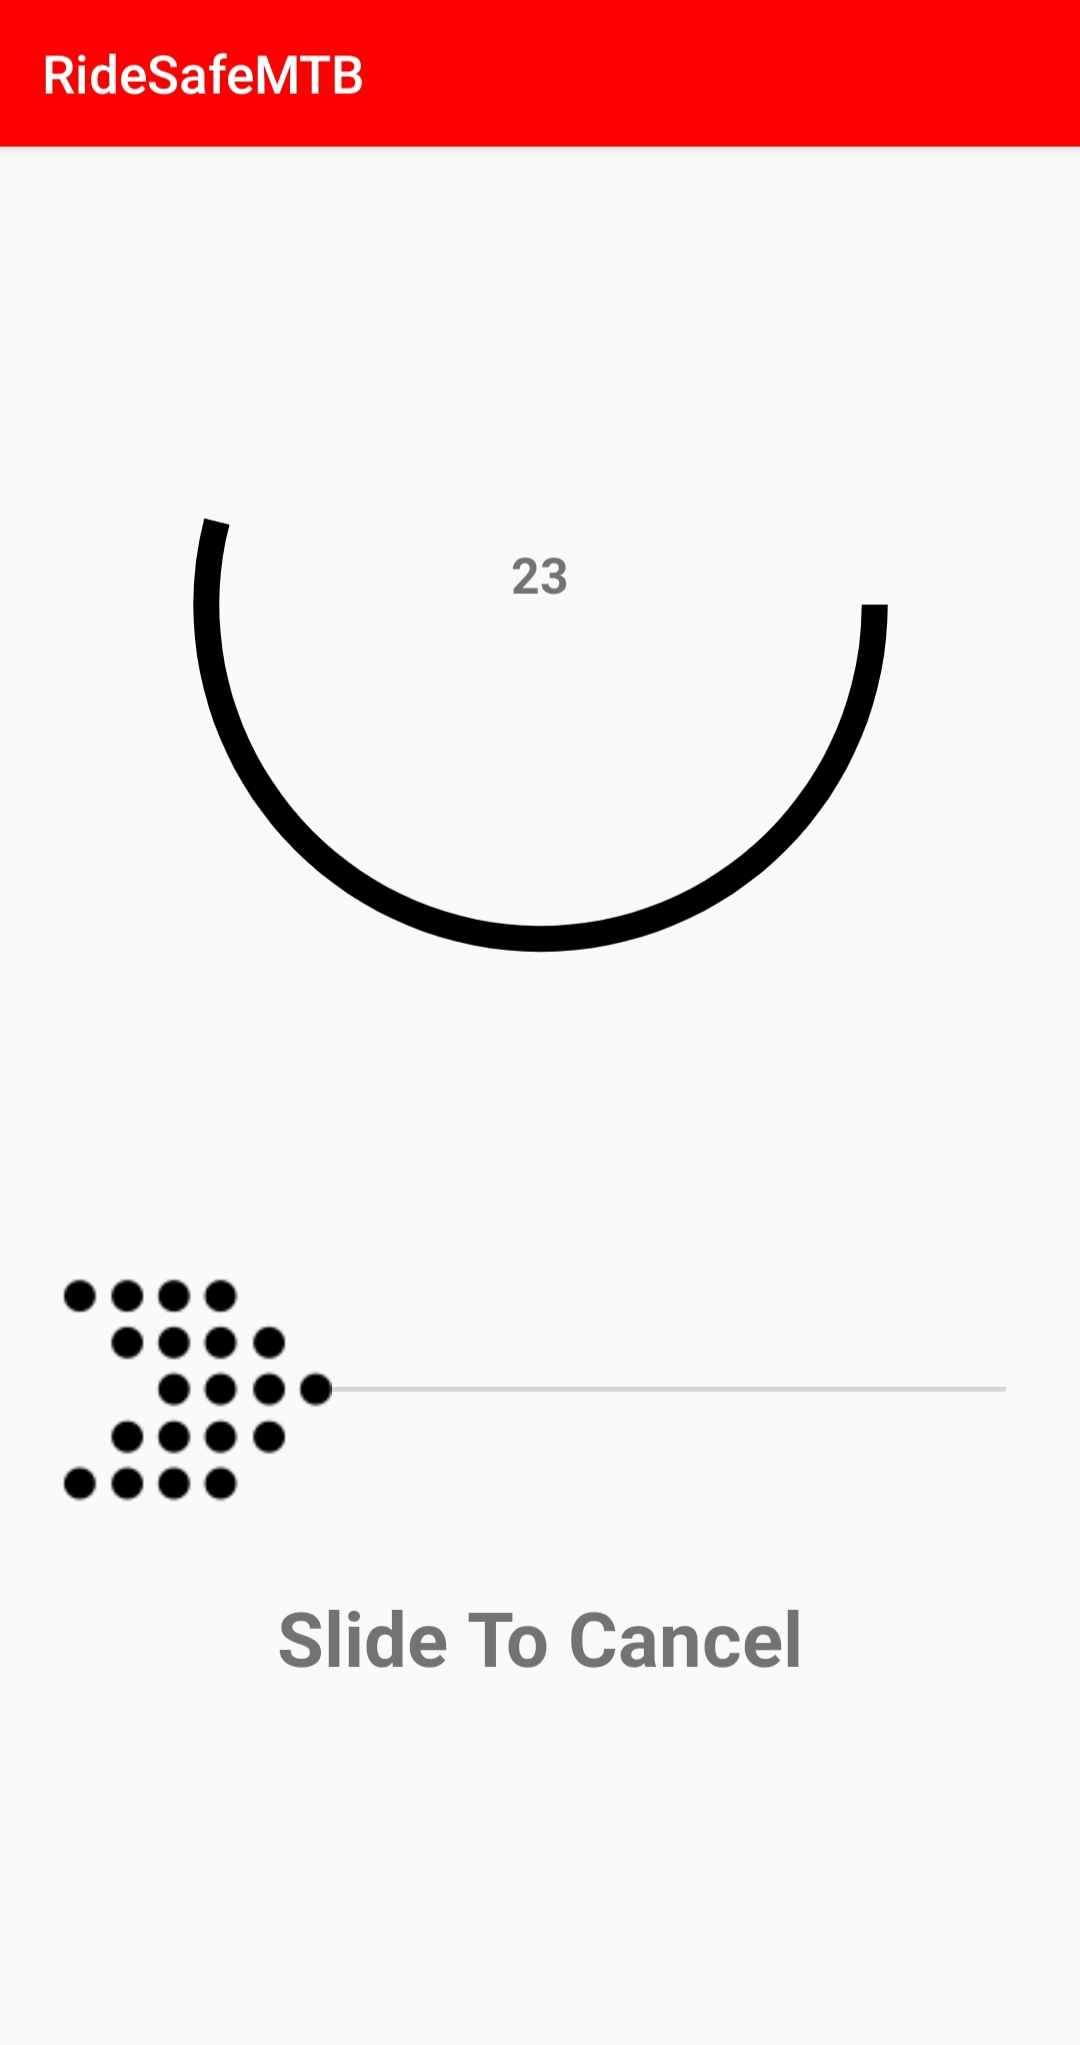
\includegraphics[scale = 0.15] {implementation/crash.jpg}
\end{center}
\caption{A Screenshot of the Crash Handler}
\label{crash}
\end{wrapfigure}
%%%%%%%%%%%%%%%%%%%%%%%%%%%%%%%%%%%%%%%%



figure \ref{crash} shows the layout of the crash handling screen, The crash handler is launched by means of an intent from the background service previously discussed as shown below. The location and speed of where the crash occurred is passed via a bundle for usage in both the accident heatmap and for content in the automatic SMS which is sent.

 \begin{lstlisting}[language=Java,basicstyle=\small, breaklines=true, label={lst:labell},caption={Launching the Crash Handler}]



void LaunchCrashHandler(){
        Intent intent = new Intent(RideSafeService.this, Crash_Handler.class).setFlags(Intent.FLAG_ACTIVITY_NEW_TASK);
        Bundle b = new Bundle();
        b.putDouble("latitude", current.getLatitude());
        b.putDouble("longitude", current.getLongitude());
        b.putDouble("speed", SPEEDCURR);
        intent.putExtras(b);
        startActivity(intent);

    }


\end{lstlisting}

As the crash handler is launched while the users phone is  out of hand and the device locked, extra flags were set for the activity so that it can be launched and displayed from a locked device. By passing the users lockscreen the crash handler is displayed an an audible alarm is played on repeat.Password,pin entry or fingerprint scanning is all bypassed when the activity is launched. The alarm is for the scenario where a false positive my occur to alert the rider to cancel the timer before the sms is sent.
The flags used were as follows:
 \begin{lstlisting}[language=Java,basicstyle=\small, breaklines=true, label={lst:labell},caption={Flags to allow device to RideSafe to display the crash handler}]




 this.getWindow().setFlags(WindowManager.LayoutParams.FLAG_FULLSCREEN |
                        WindowManager.LayoutParams.FLAG_DISMISS_KEYGUARD |
                        WindowManager.LayoutParams.FLAG_SHOW_WHEN_LOCKED |
                        WindowManager.LayoutParams.FLAG_TURN_SCREEN_ON,
                WindowManager.LayoutParams.FLAG_FULLSCREEN |
                        WindowManager.LayoutParams.FLAG_DISMISS_KEYGUARD |
                        WindowManager.LayoutParams.FLAG_SHOW_WHEN_LOCKED |
                        WindowManager.LayoutParams.FLAG_TURN_SCREEN_ON);

\end{lstlisting}


While the alarm is played, a countdown timer is displayed on screen along with a slide bar used to cancel the countdown. In the event of a false positive or an accident where the rider does not require assistance, sliding the cancel slider will cancel the timer and relaunch the background service and re locking the device. A slider is used as it is much more unlikely to accidentally slide to cancel compared to just pressing  a button.


Once the timer expires the users chosen emergency contact is automatically sent an SMS e, g,.  I have had an accident. my location is :https://maps.google.com/?q=" + Latitude + "," + Longitude   "I Crashed while traveling at : " + Speed + "kmph   Sent Automatically by RideSafe".   The users speed and location which were passed from the service intent are used to automatically generate a link to their location on google maps, allowing the emergency contact to relay the information to the authorities, or simply by clicking the link receive directions to accident site themselves. 

 \begin{lstlisting}[language=Java,basicstyle=\small, breaklines=true, label={lst:labell},caption={Automatic SMS Sending}]


private void sendSms() {
        SmsManager smsManager = SmsManager.getDefault();
        smsManager.sendTextMessage(PhoneNumber, null, message, null, null);
        Toast.makeText(getApplicationContext(), "SMS sent to " + ContactName,
                Toast.LENGTH_LONG).show();


    }
\end{lstlisting}


\newpage


\subsection{Settings}

%%%%%%%%%%%%%%%%%%%%%%%%%%%%%%%%%%%%%%%%
\begin{wrapfigure}{r}{0.3\textwidth}
\begin{center}
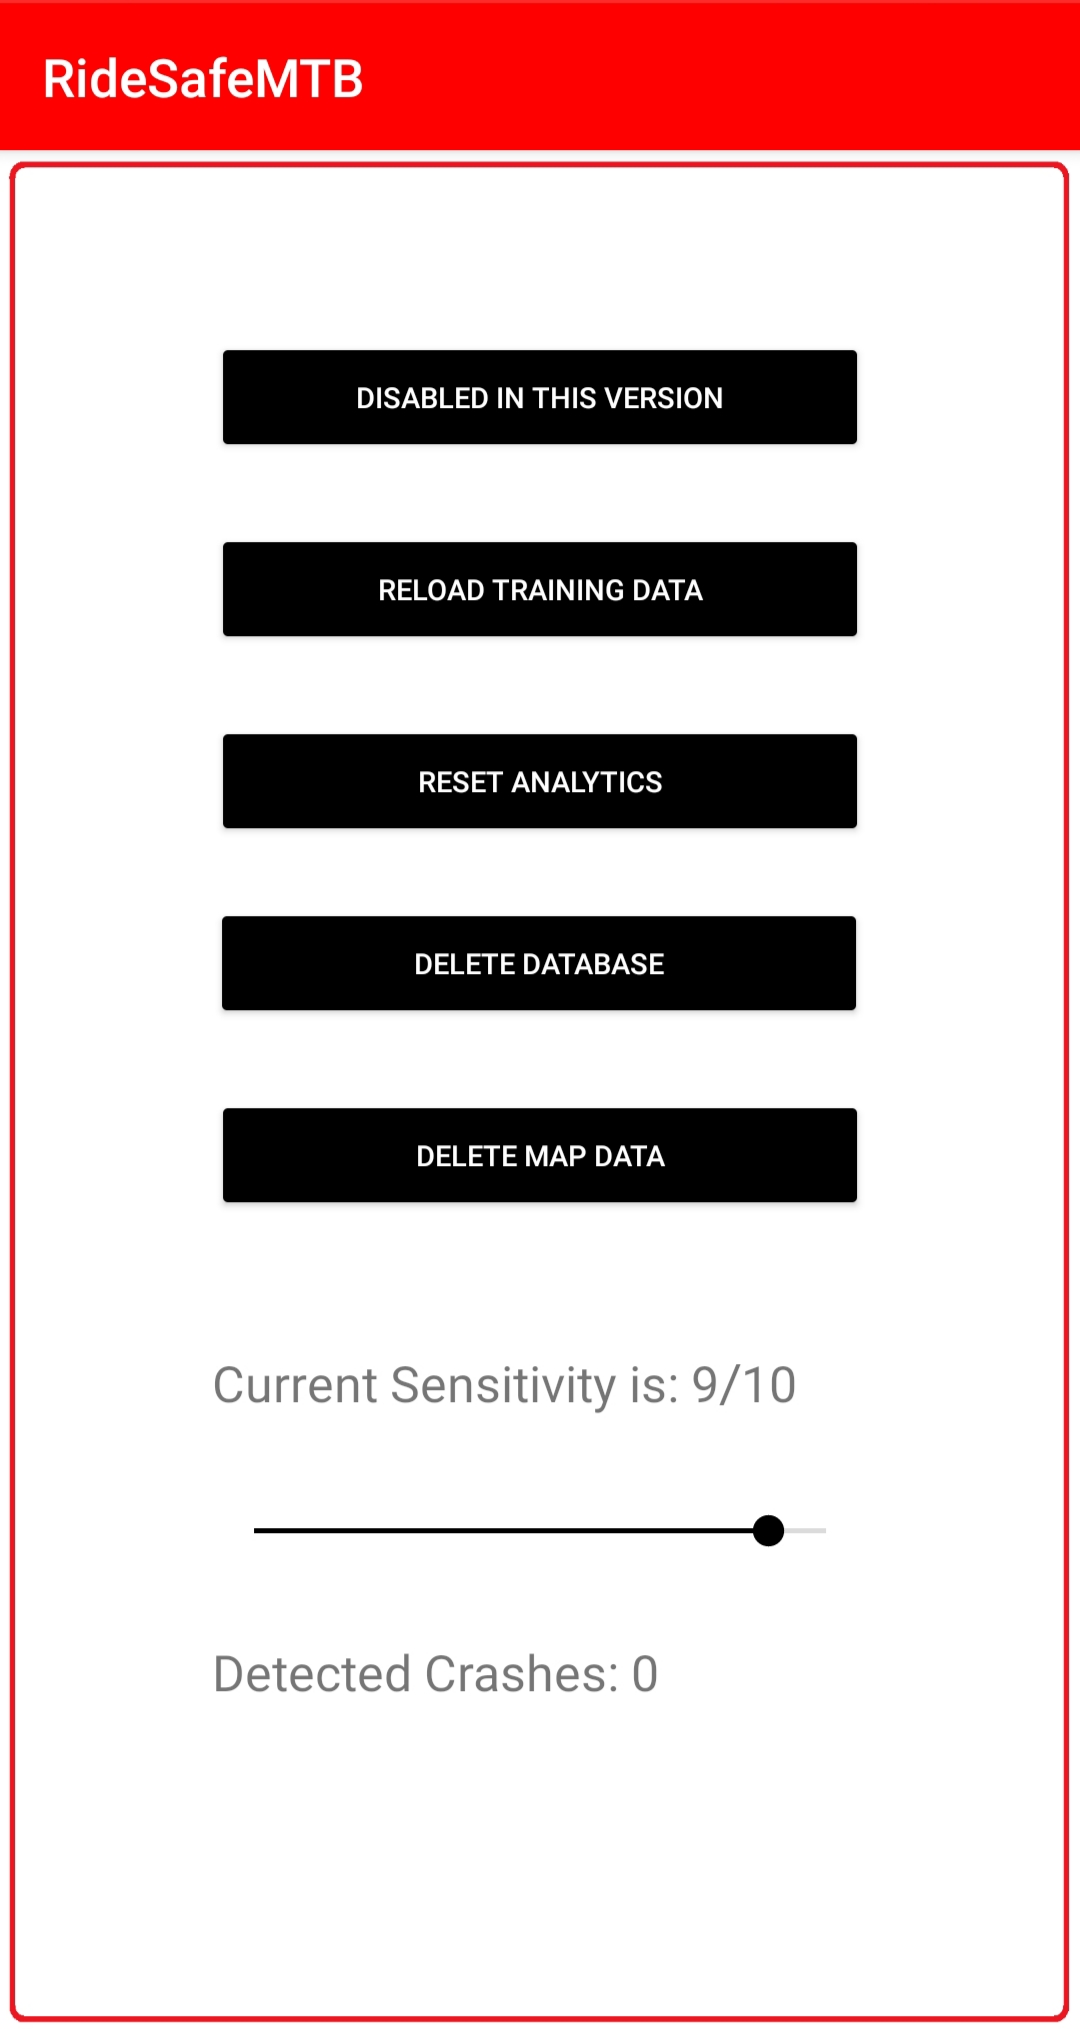
\includegraphics[scale = 0.15] {implementation/set.jpg}
\end{center}
\caption{A Screenshot of the Settings Screen}
\label{set}
\end{wrapfigure}
%%%%%%%%%%%%%%%%%%%%%%%%%%%%%%%%%%%%%%%%

The settings screen as seen in Figure \ref{set}, provides a few useful functions to the end user:

As this screenshot is from the version currently listed on google play the function “export data to the developer” has been disabled in the store version.  The button was originally implemented for allowing quick transfering of sensor data. Upon pressing the button the full database of RideSafe was saved as a database file which was sharable in the android operating system. Data could easily be transferred via email for debugging purposes. Delete Database is closely related and was used in conjunction with the export button to allow small samples of data to be recorded and then deleted, allowing for small separate files rather than a single large file to be exported.

Reload Training data is a manual override to reload and re train the system,  When crashes occur the values associated are added to the systems database, at a convenient time for the user the values are added to the classifier and the system can be retrained.

Reset Analytics and Delete map data are both implemented to clear user specific data such as previous journey latitudes and longitudes used to plot journeys on the map or the max speed displayed on the home screen.

As mentioned in the discussion of the background service, there exists a threshold value for the probability required to trigger a detected crash, the settings screen includes a sensitivity slider to adjust the threshold value used. Each notch on the slider increments or decrements this value by .05, allowing users slight adjustment to improve their experience while using the supplied training data.

The detected crash counter, used for testing purposes is a counter of how many times the application has detected an accident. 


\section{Non-Functional Requirements Implemented}
\vspace{3cm}


%%%%%%%%%%%%%%%%%%%%%%%%%%%%%%%%%%%%%%%%
\begin{figure}[h]
      \centering
      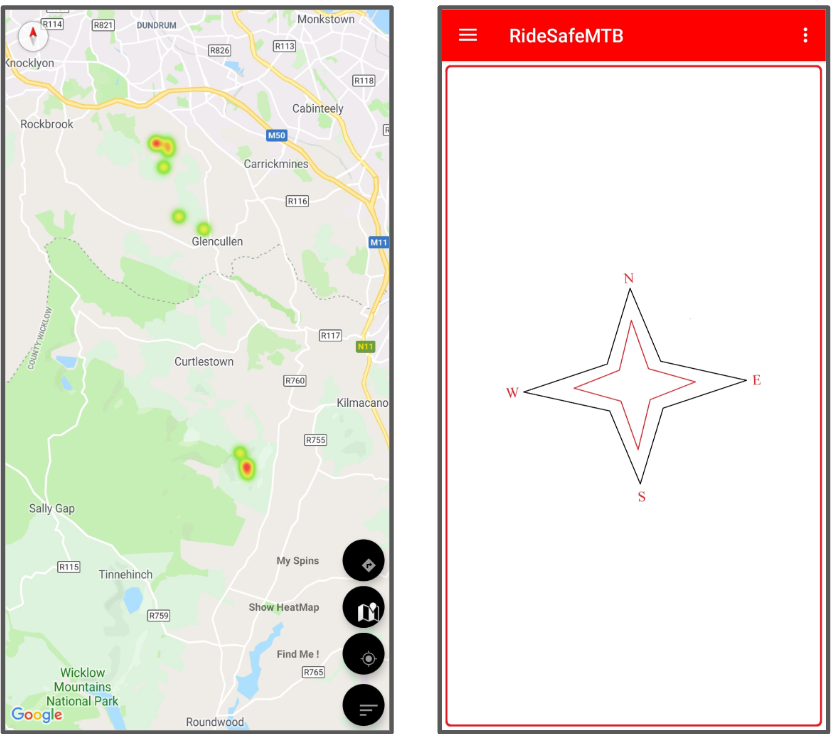
\includegraphics[scale = .9]{implementation/cm.png}
      \caption{Accident HeatMap (left), Compass (Right)}
      \label{cm}
\end{figure}
%%%%%%%%%%%%%%%%%%%%%%%%%%%%%%%%%%%%%%%%

\subsection{Google Maps}

Google's map API was taken utilized to implement two additional features:
\begin{itemize}
\item Accident heatmap 
\end{itemize}

Users can currently see potential danger zones where previous accidents have occured. Once a crash has been detected the users latitude and longitude of where the crash has occurred is plotted on RideSafes built in map. As the size and colour of the spot on the map increases the likelihood of present danger increases. By viewing the map users could decide to take extra caution while passing through the area, or avoid it entirely, potentially preventing an accident occurring. Currently the heatmap is user specific, future plans for the heatmap will be discussed in future work.   

\begin{itemize}
\item Ride Tracking
\end{itemize}
A Simple way to view trails and journeys ridden by the user. By storing the latitudes and longitudes where the rider has travelled in a database table, these points can be plotted on the map allowing the user to view places they have been and passed by. The speed of which the rider was travelling at the certain locations was also recorded with the intention to change the colour of the plotted journey according to the recorded speed however, due to time constraints dynamic line colouring has yet to be implemented.





\subsection{Compass}





With Certain trails being situated in very remote areas, navigation can sometimes be an issue, especially when a connection to the internet cannot be obtained. Using the orientation sensor the direction of magnetic north can be calculated. By simply rotating an image with offsets calculated to point north a very simple yet reliable compass has been implemented. A small but useful feature.








\section{Training}



The Logistic model utilized in RideSafe has been trained by collecting training data in two seperate ways:
\begin{itemize}
\item Logging of ride Data 
\end {itemize}

In the early stages of development data was collected solely by the author while mountain biking at local trail centres. Similar to medical solutions the “ADL” of mountain biking had to be identified and the patterns learnt. Globally trails are allocated a rating to how technical and difficult they are, ranging from a “green” trail to “double black diamond”. Thousands of points of data were collected from “blue” “red” \& “black” trails in the Dublin/Wicklow area. This data proved invaluable in terms of learning what are considered “normal” sensor readings while mountain biking. Upon receiving ethical approval data has been collected from numerous riders of varying skill level and experience.
\begin{itemize}
\item Crashing in a controlled environment
\end{itemize}
For the model not to be biased an equal number of instances of both crash data and non crash data must be present in the training data, With few “real World” major accidents occurring during the data collection phase action was taken to ensure the system could be trained correctly. Alike the training performed in medical applications where controlled falls are purposely done onto a soft surface such as a mattress, the author conducted similar tests at the local indoor skate park.
Three hours of intentional crashes were performed in one of two main ways: The most common cause of severe mountain biking injury - over the handlebars as well as side impact which is commonly caused by loss of traction.    







Figure \ref{fall} shows stills of a video taken with accompanying sensor readings closely aligned. The sample rate used was 3 readings of each sensor per second bar speed which is slower to calculate ( roughly once per second). The data readings are labelled and are displayed over time.
 The first section closely resembles data collected from normal riding on a green trail, slow speed, low g-force and marginal rotation of the device. 
Section 2 closely resembles data collected from riding blue/red trails, spikes in both g-force and rotation of the device, more movement in terms of rotational velocity on all axis as well as spikes in g-force. In this instance the spikes are caused by the small direction change associated riding the takeoff ramp.
Section 3 \& 4 are of most interest, the flatline from the sensor values are caused by gliding through the air, completely off the ground. Section 4 is both impact and aftermath. Big spikes of both g-force and rotational velocity can be observed as impact occurs. As clear from the graph the change in speed is a huge anomaly compared to standard riding. The results of this testing allowed for the development of RideSafe’s rule base.

After countless intentional falls enough data was collected to both identify the characteristics and pattern of the events occuring during an accident.  




%%%%%%%%%%%%%%%%%%%%%%%%%%%%%%%%%%%%%%%%
\begin{figure}[h]
      \centering
      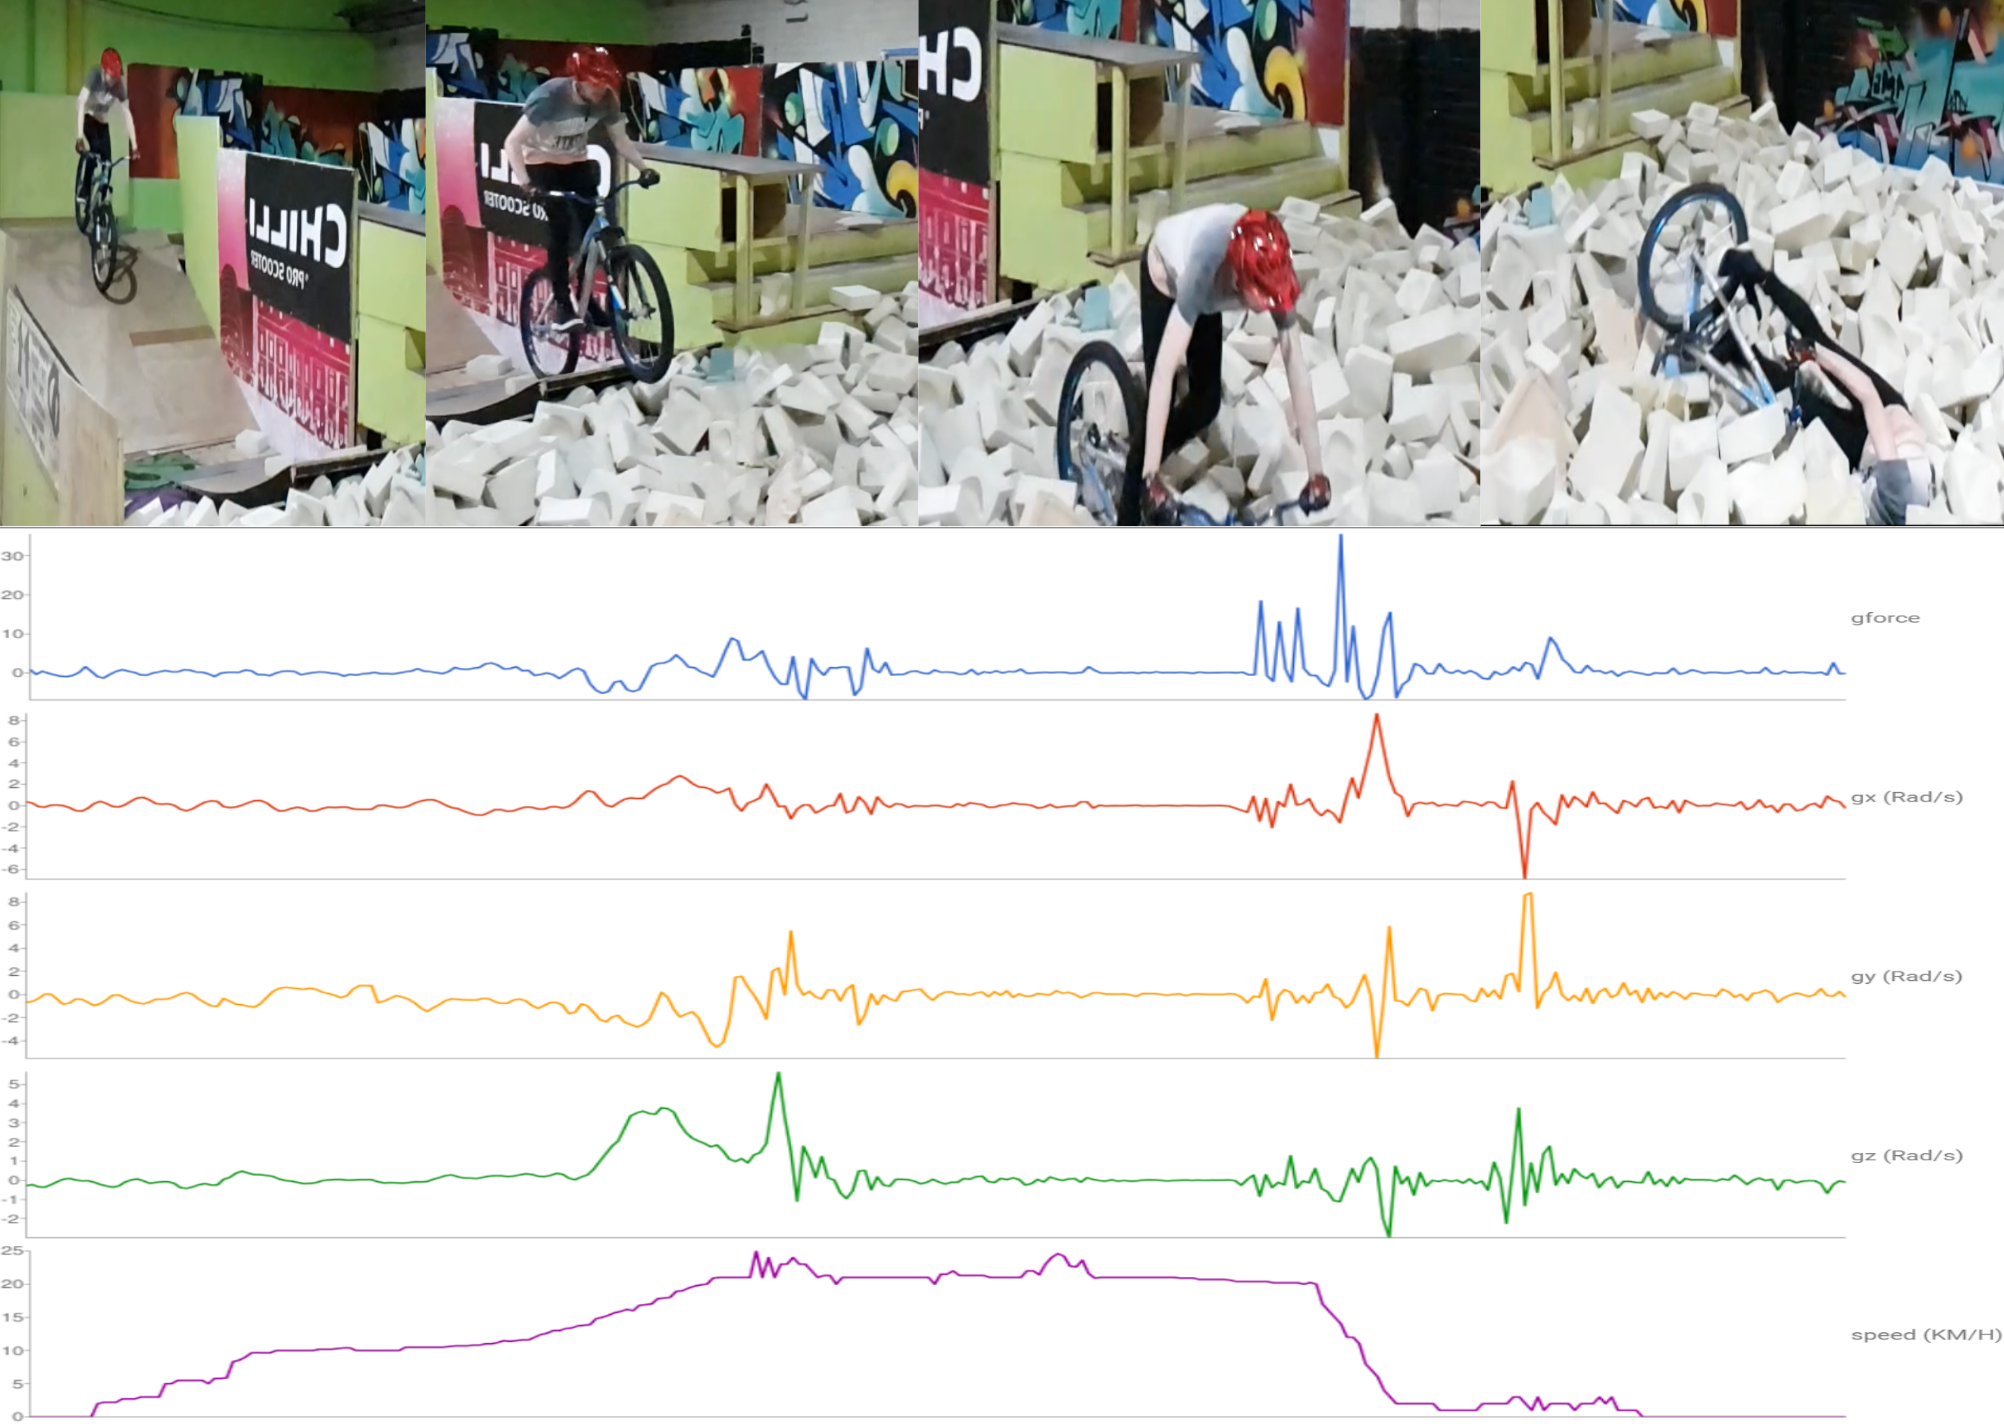
\includegraphics[scale = .6]{implementation/fall.png}
      \caption{Analysis of A Crash}
      \label{fall}
\end{figure}
%%%%%%%%%%%%%%%%%%%%%%%%%%%%%%%%%%%%%%%%SS

\newpage
\section {Application Flow Diagram}


%%%%%%%%%%%%%%%%%%%%%%%%%%%%%%%%%%%%%%%%
\begin{figure}[h]
      \centering
      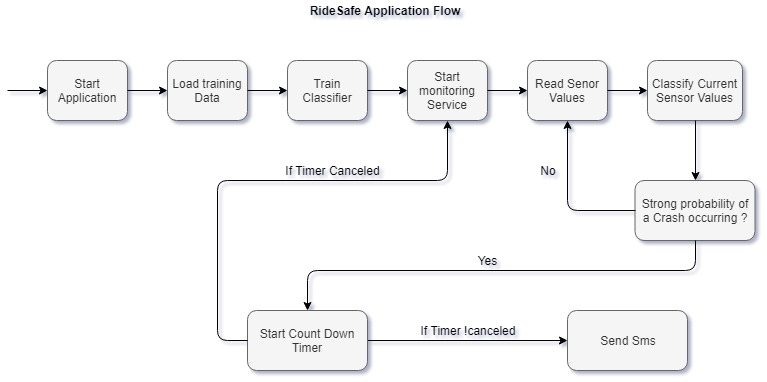
\includegraphics[scale = .6]{implementation/flow.jpg}
      \caption{RideSafe Application Flow}
      \label{flow1111}
\end{figure}
%%%%%%%%%%%%%%%%%%%%%%%%%%%%%%%%%%%%%%%%SS






